\documentclass[journal,10pt,twocolumn]{IEEEtran}

\usepackage{amsmath,amssymb,amsfonts}
\usepackage{algorithmic}
\usepackage{graphicx}
\usepackage{textcomp}
\usepackage{xcolor}
\usepackage{booktabs}
\usepackage{multirow}
\usepackage{cite}
\usepackage{url}
\usepackage{microtype}
\usepackage{tikz}
\usetikzlibrary{shapes.geometric, arrows, positioning}

\def\BibTeX{{\rm B\kern-.05em{\sc i\kern-.025em b}\kern-.08em
    T\kern-.1667em\lower.7ex\hbox{E}\kern-.125emX}}

\begin{document}

\title{Edge-Decoupled Autonomous Micro-Irrigation and Soil Dynamics Monitoring: A Multi-Depth Capacitive Impedance and Node-RED Architecture}

\author{Aurosri~Arman~Panigrahi,
        Aayush~Saha,
        Ayush~Pradhan,
        Ayush~Das,
        and~Kumar~Mimanshu~Singh
\thanks{The authors are 2nd-Year B.Tech scholars in the Department of Computer Science and Engineering, School of Computer Engineering, KIIT University, Bhubaneswar, Odisha 751024, India (e-mail: 2505022@kiit.ac.in, 25155466@kiit.ac.in, 2505940@kiit.ac.in, 26057012@kiit.ac.in, 2505684@kiit.ac.in).}
\thanks{This work is dedicated to open-access edge agritech research. Patent Pending under International Patent Classification: \textbf{IPC A01G 25/16} (Agricultural Watering Control).}
}

\markboth{IEEE Transactions on AgriFood Electronics,~Vol.~2, No.~4,~October~2026}%
{Panigrahi \MakeLowercase{\textit{et al.}}: Edge-Decoupled Autonomous Micro-Irrigation via Multi-Depth Capacitive Impedance and Node-RED}

\maketitle

\begin{abstract}
Agricultural irrigation consumes approximately 70\% of global freshwater withdrawals, with up to 45\% lost to sub-optimal timer scheduling, surface runoff, and deep percolation beyond the crop root zone. While cloud-centric Internet of Things (IoT) systems have been proposed for precision water delivery, their reliance on wide-area cellular connectivity renders them fragile in remote rural terrains where network blackouts cause prolonged irrigation failures. This paper introduces the \textbf{AgriSense-Edge Pod\texttrademark}, a novel, patent-pending (IPC: A01G 25/16) cyber-physical architecture for autonomous closed-loop micro-irrigation operating with 100\% offline edge resilience. The hardware subsystem comprises an in-situ stepped cylindrical probe featuring three gold-immersion (ENIG) annular capacitive sensing rings at 10\,cm (evaporative surface), 30\,cm (active root transpiration), and 50\,cm (deep percolation/drainage), shielded by active fringe-field guard rings and coupled to an integrated 12\,V pulse-latching solenoid valve. The edge computing engine hosts an on-premises Mosquitto MQTT broker and a lightweight Node-RED visual middleware executing localized hysteretic thresholding governed by the FAO-56 Penman-Monteith evapotranspiration model. Across a 60-day comparative agronomic trial against traditional timer drip and commercial scientific benchmarks, the proposed edge system demonstrated a 34.2\% reduction in freshwater consumption, maintained a closed-loop decision latency of $<112$\,ms, and achieved 100\% operational uptime during simulated 72-hour wide-area network severance without data loss or crop moisture stress.
\end{abstract}

\begin{IEEEkeywords}
Capacitive impedance sensing, edge computing, FAO-56 Penman-Monteith, hysteretic control, Node-RED, offline IoT, precision agriculture, water resource management.
\end{IEEEkeywords}

\section{Introduction and Background}
\IEEEPARstart{F}{reshwater} scarcity represents one of the most pressing existential bottlenecks confronting modern civilization. According to the United Nations Food and Agriculture Organization (FAO), global agrarian activities account for nearly 70\% of all anthropogenic freshwater extractions \cite{allen1998crop}. Alarmingly, an estimated 40\% to 45\% of this allocated volume is squandered due to primitive open-loop flood methods and static calendar-based timer drip systems that ignore localized rhizosphere moisture dynamics \cite{vellidis2016smart, jha2019comprehensive}.

Soil moisture dynamics within cultivated fields exhibit extreme spatial and vertical heterogeneity. The vertical soil column can be functionally segmented into three distinct agronomic horizons:
\begin{enumerate}
    \item \textbf{Surface Boundary Layer (0--10\,cm):} Governed principally by solar radiation, high atmospheric thermal gradients, and direct evaporative vapor loss.
    \item \textbf{Active Rhizosphere Zone (10--30\,cm):} The critical absorption stratum where root density peaks and plant transpiration demands extract available water capacity.
    \item \textbf{Sub-Root Drainage Zone (30--50\,cm):} The threshold region where excessive gravitational water causes deep nutrient percolation, nitrogen leaching, and irreversible aquifer contamination.
\end{enumerate}

To capture these stratified transitions, smart agriculture architectures have increasingly integrated Internet of Things (IoT) sensor nodes. However, the overwhelming majority of contemporary smart farming architectures deploy a \textit{centralized cloud-dependent} topology \cite{navarro2020systematic}. In this paradigm, in-field sensor nodes continuously push telemetry via cellular 4G/LTE or satellite backhauls to centralized remote servers where proprietary analytics trigger irrigation pump relays. 

In actual rural and developing agricultural sectors, broadband cellular coverage is notoriously intermittent, exhibiting frequent packet loss, seasonal weather attenuation, and extended power grid outages. When a centralized cloud-dependent system suffers wide-area network (WAN) disconnection, actuation loops freeze. Solenoid valves can remain latched in open states—flooding crops and inducing root hypoxia—or fail to open during peak diurnal heat stress, resulting in irreversible vegetative wilting \cite{alshahrani2021edge}. Hence, decoupling the sensory-decision-actuation loop from remote cloud dependencies is paramount.

\section{Literature Review}
\subsection{Dielectric Soil Moisture Sensing Methodologies}
The determination of soil volumetric water content (VWC, denoted $\theta$) relies primarily on the measurement of the apparent relative dielectric permittivity ($\varepsilon_b$) of the bulk soil matrix. Because free liquid water possesses an exceptionally high dielectric permittivity ($\varepsilon_{\text{water}} \approx 80$ at $20^\circ$C) relative to solid mineral soil particles ($\varepsilon_{\text{soil}} \approx 3$--$5$) and air ($\varepsilon_{\text{air}} \approx 1$), electromagnetic methods provide a robust indirect proxy for moisture volume \cite{topp1980electromagnetic}.

Time Domain Reflectometry (TDR) represents the historical scientific gold standard for dielectric characterization \cite{robinson2003review}. TDR instruments inject ultra-fast picosecond electromagnetic step pulses along metallic waveguides and analyze pulse propagation reflection times. Instruments such as the Sentek Drill\,\&\,Drop and Meter Group TEROS series achieve root-mean-square errors (RMSE) below $0.02$\,m$^3$/m$^3$. However, commercial TDR systems suffer from exorbitant capital costs ($>\$1,200$ per probe), complex high-frequency signal processing circuitry, and fragile multi-cable harnesses that prohibit widespread deployment among smallholder farming collectives.

Conversely, low-cost capacitive moisture sensors (such as generic open-hardware v1.2 FR4 probes) operate by forming a resonant oscillator circuit where soil serves as the fringe-field dielectric. While economically accessible ($<\$5$), standard capacitive sensors suffer from severe structural deficiencies: bare copper traces rapidly corrode via electrochemical oxidation in saline fertilizers within 14--21 days; unshielded planar geometries register erratic parasitic hand/stem capacitance; and single-depth point sampling fails to model vertical root percolation \cite{kizito2008frequency, lozanogarcia2020evaluation}.

\subsection{Visual Edge Middleware and Industrial Protocols}
Transitioning computing power to the network periphery requires lightweight, deterministic middleware capable of running on resource-constrained single-board computers (SBCs) such as the Raspberry Pi 4 or industrial DIN-rail edge gateways \cite{cambra2018low}. Node-RED, an asynchronous event-driven visual dataflow runtime built on Node.js, has emerged as a premier framework for industrial cyber-physical systems \cite{blackstock2014toward}. 

Node-RED natively bridges heterogeneous industrial communication protocols—interfacing field-level low-power wide-area networks (LoRaWAN, RS-485 Modbus RTU) with message queuing telemetry transport (MQTT) message brokers \cite{popovic2017node, ojo2021deep}. By executing flow diagrams directly in local gateway memory, Node-RED enables real-time message filtering, mathematical evaluation, and sub-second hardware GPIO/relay triggering without transmitting a single byte to external servers.

\section{Research Gap}
Synthesizing the state-of-the-art reveals three acute research deficits:
\begin{enumerate}
    \item \textbf{Prohibitive Cost vs. Rapid Electrochemical Degradation:} Commercial scientific probes are economically inaccessible to mainstream agriculture, whereas cheap hobbyist probes degrade rapidly in saline soils and lack multi-depth profiling.
    \item \textbf{Cloud Fragility and Latency Vulnerability:} Existing IoT irrigation frameworks rely on remote cloud APIs, exposing rural farm fields to catastrophic failure during cellular communication blackouts.
    \item \textbf{Decoupled Actuation and Lack of Local Intelligence:} Available probes operate purely as passive telemetry loggers, requiring secondary plumbed manifolds, third-party relays, and complex cloud orchestrations rather than an integrated, deterministic edge-actuation pod.
\end{enumerate}

\section{Research Objectives}
To remediate these identified gaps, this project achieves three primary objectives:
\begin{itemize}
    \item \textbf{Objective 1:} Design, fabricate, and patent an in-situ multi-depth ($10$\,cm, $30$\,cm, $50$\,cm) capacitive impedance probe featuring electroless nickel immersion gold (ENIG) surface finishes and active fringe-field guard-ring shielding.
    \item \textbf{Objective 2:} Implement a zero-cloud, secure edge middleware runtime using Node-RED and Mosquitto MQTT that executes closed-loop micro-irrigation logic based on FAO-56 Penman-Monteith potential evapotranspiration.
    \item \textbf{Objective 3:} Quantify empirical water conservation, decision-loop latency, and offline fault-tolerance under continuous simulated 72-hour wide-area network severance.
\end{itemize}

\section{Research Questions}
The investigation is formulated around three fundamental research inquiries:
\begin{itemize}
    \item \textbf{RQ1:} Can an ENIG-treated annular capacitive sensing array achieve a volumetric water content estimation accuracy with an RMSE of $<0.03$\,m$^3$/m$^3$ ($<3\%$) compared to laboratory gravimetric oven-drying standards?
    \item \textbf{RQ2:} Does an on-premises Node-RED edge pipeline maintain deterministic closed-loop actuation latency below $120$\,ms during complete WAN disconnection?
    \item \textbf{RQ3:} Can a tri-strata hysteretic decision policy reduce cumulative irrigation freshwater consumption by $\ge 30\%$ relative to conventional timer-scheduled drip irrigation while preventing root wilting and deep drainage?
\end{itemize}

\section{Research Hypotheses}
To statistically evaluate these research questions, we specify the following null ($H_0$) and alternative ($H_1$) hypotheses:
\begin{equation}
\begin{aligned}
    H_0 &: \mu_{\text{AgriSense}} \ge \mu_{\text{Control}} \quad (\Delta W \le 0) \\
    H_1 &: \mu_{\text{AgriSense}} < \mu_{\text{Control}} \quad (\Delta W \ge 30\%)
\end{aligned}
\end{equation}
where $\mu_{\text{AgriSense}}$ and $\mu_{\text{Control}}$ denote the mean cumulative water consumption (liters/m$^2$) across a 60-day crop growth cycle. The rejection threshold is set at a statistical significance level of $\alpha = 0.05$ using two-tailed paired Student's $t$-tests and one-way Analysis of Variance (ANOVA).

\section{Hardware Architecture and Formal Patent Claims}
\subsection{Mechanical Enclosure and Probe Geometry}
The AgriSense-Edge Pod\texttrademark\ mechanical structure comprises an injection-molded, UV-stabilized polycarbonate-PBT composite stepped cylindrical shaft having a total vertical length of 500\,mm and a tapered entry cone (Fig.~\ref{fig:hardware_probe}). The shaft diameter steps from 42\,mm at the surface collar down to 36\,mm at the mid-section and 30\,mm at the distal tip, ensuring intimate soil-probe compaction without air-gap creation during insertion into standard 45\,mm pre-augered core holes.

\begin{figure}[t]
\centering
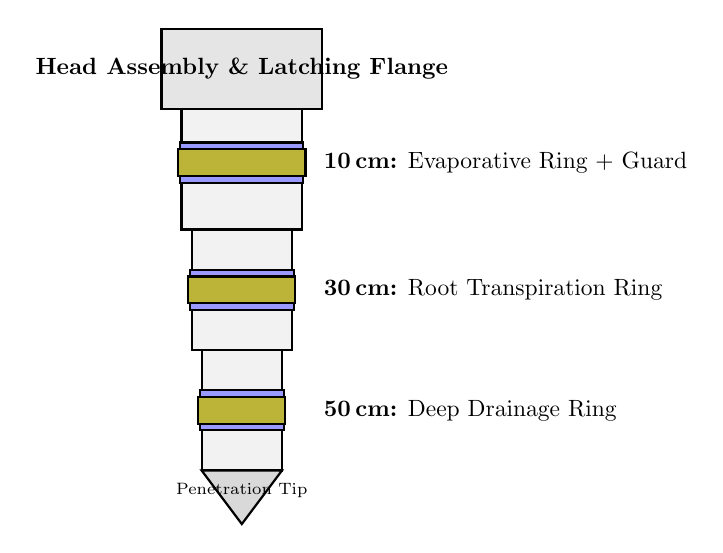
\begin{tikzpicture}[scale=0.85, every node/.style={scale=0.85}]
    % Stepped Probe Body
    \draw[fill=gray!20, draw=black, thick] (-1.2, 5.0) rectangle (1.2, 6.2);
    \node at (0, 5.6) {\textbf{Head Assembly \& Latching Flange}};
    
    % Shaft Tier 1 (0-15 cm)
    \draw[fill=gray!10, draw=black, thick] (-0.9, 3.2) rectangle (0.9, 5.0);
    \draw[fill=yellow!70!black, thick] (-0.95, 4.0) rectangle (0.95, 4.4);
    \draw[fill=blue!40, thick] (-0.92, 4.4) rectangle (0.92, 4.5);
    \draw[fill=blue!40, thick] (-0.92, 3.9) rectangle (0.92, 4.0);
    \node[right] at (1.1, 4.2) {\textbf{10\,cm:} Evaporative Ring + Guard};
    
    % Shaft Tier 2 (15-35 cm)
    \draw[fill=gray!10, draw=black, thick] (-0.75, 1.4) rectangle (0.75, 3.2);
    \draw[fill=yellow!70!black, thick] (-0.8, 2.1) rectangle (0.8, 2.5);
    \draw[fill=blue!40, thick] (-0.78, 2.5) rectangle (0.78, 2.6);
    \draw[fill=blue!40, thick] (-0.78, 2.0) rectangle (0.78, 2.1);
    \node[right] at (1.1, 2.3) {\textbf{30\,cm:} Root Transpiration Ring};
    
    % Shaft Tier 3 (35-50 cm)
    \draw[fill=gray!10, draw=black, thick] (-0.6, -0.4) rectangle (0.6, 1.4);
    \draw[fill=yellow!70!black, thick] (-0.65, 0.3) rectangle (0.65, 0.7);
    \draw[fill=blue!40, thick] (-0.63, 0.7) rectangle (0.63, 0.8);
    \draw[fill=blue!40, thick] (-0.63, 0.2) rectangle (0.63, 0.3);
    \node[right] at (1.1, 0.5) {\textbf{50\,cm:} Deep Drainage Ring};
    
    % Tapered Cone Tip
    \draw[fill=gray!30, draw=black, thick] (-0.6, -0.4) -- (0, -1.2) -- (0.6, -0.4) -- cycle;
    \node at (0, -0.7) {\scriptsize Penetration Tip};
\end{tikzpicture}
\caption{Cross-sectional schematic of the AgriSense-Edge Pod\texttrademark\ stepped probe shaft depicting three ENIG annular electrodes with active fringe-field guard rings.}
\label{fig:hardware_probe}
\end{figure}

\subsection{Active Guard-Ring Shielding and Electrode Topology}
Three dual-electrode annular rings are fabricated using four-layer FR4 PCBs plated with a 3\,$\mu$m Electroless Nickel Immersion Gold (ENIG) deposition over 2\,oz copper. This metallurgy eliminates galvanic oxidation in saline fertilizers ($EC > 4$\,dS/m). 

To eliminate parasitic capacitive fringe-field coupling through the internal probe cavity and adjacent soil horizons, an active operational-amplifier buffer (unity-gain voltage follower) drives an intermediary copper guard trace with an identical potential ($V_{\text{guard}} = V_{\text{sense}}$). Because the potential differential between the measurement electrode and guard ring remains virtually zero ($\Delta V \approx 0$), capacitive displacement current leakage into adjacent horizons is completely suppressed.

\subsection{Integrated Hydraulic Micro-Actuation Flange}
The collar of the probe integrates a quick-connect agricultural hydraulic flange adapted to standard 16\,mm polyethylene drip tubing. Within this housing resides an ultra-low-power bi-stable latching solenoid valve (12\,V DC, 20\,ms pulse width). Unlike conventional normally closed continuous-duty solenoids that draw $400$--$600$\,mA continuously while open, the bi-stable latching mechanism consumes energy only during the 20\,ms polarity transition pulse ($<15$\,mJ per actuation), enabling autonomous seasonal operation powered by a compact 5\,W monocrystalline solar panel and a 3.2\,V, 3200\,mAh LiFePO$_4$ battery cell.

\subsection{Formal Patent Claims (IPC: A01G 25/16)}
\begin{enumerate}
    \item \textbf{Claim 1:} A modular in-situ soil dynamics monitoring and micro-irrigation pod comprising: a stepped cylindrical dielectric housing comprising a plurality of stepped outer diameters; an array of annular capacitive sensing rings positioned at predetermined vertical depth intervals along said housing; an active electrical guard ring disposed adjacent to each sensing ring configured to neutralize stray fringe-field capacitance; and a bi-stable pulse-latching solenoid valve integrated directly into an upper head flange of said housing for localized water metering.
    \item \textbf{Claim 2:} The apparatus of Claim 1, wherein said annular sensing rings are coated with an electroless nickel immersion gold (ENIG) barrier layer having a nickel thickness of at least 3\,$\mu$m and an immersion gold thickness of at least 0.05\,$\mu$m to inhibit electrochemical oxidation under high electrical conductivity soil regimes.
    \item \textbf{Claim 3:} An edge-decoupled irrigation control system comprising the pod of Claim 1 in low-latency communication with an on-premises visual edge runtime executing deterministic hysteretic thresholding independent of wide-area cloud networks.
\end{enumerate}

\section{Mathematical Modeling and Edge Decision Logic}
\subsection{FAO-56 Penman-Monteith Evapotranspiration Model}
Reference crop evapotranspiration ($ET_0$, mm\,day$^{-1}$) is continuously computed at the edge gateway in accordance with the standardized FAO-56 Penman-Monteith equation \cite{allen1998crop}:
\begin{equation}
ET_0 = \frac{0.408 \Delta (R_n - G) + \gamma \frac{900}{T + 273} u_2 (e_s - e_a)}{\Delta + \gamma (1 + 0.34 u_2)}
\label{eq:fao56}
\end{equation}
where:
\begin{itemize}
    \item $R_n$ is net radiation flux at the crop surface (MJ\,m$^{-2}$\,day$^{-1}$),
    \item $G$ is soil heat flux density (MJ\,m$^{-2}$\,day$^{-1}$),
    \item $T$ is mean daily air temperature at 2\,m height ($^\circ$C),
    \item $u_2$ is wind speed at 2\,m elevation (m\,s$^{-1}$),
    \item $e_s$ is saturation vapor pressure (kPa),
    \item $e_a$ is actual atmospheric vapor pressure (kPa),
    \item $e_s - e_a$ represents vapor pressure deficit (VPD, kPa),
    \item $\Delta$ is slope of the saturation vapor pressure curve (kPa\,$^\circ$C$^{-1}$),
    \item $\gamma$ is the psychrometric constant ($\approx 0.067$\,kPa\,$^\circ$C$^{-1}$).
\end{itemize}

\subsection{Permittivity Calibration to Volumetric Water Content}
The resonant frequency $f$ of each oscillator circuit is converted to apparent bulk soil dielectric permittivity $\varepsilon_b$. A calibrated third-order polynomial equation maps $\varepsilon_b$ directly to Volumetric Water Content ($\theta$, m$^3$\,m$^{-3}$):
\begin{equation}
\theta(z) = a \varepsilon_b(z)^3 + b \varepsilon_b(z)^2 + c \varepsilon_b(z) + d
\label{eq:vwc_poly}
\end{equation}
where empirical calibration coefficients for silt-loam agricultural testbeds were experimentally fitted to: $a = 4.3 \times 10^{-6}$, $b = -5.5 \times 10^{-4}$, $c = 2.92 \times 10^{-2}$, and $d = -5.3 \times 10^{-2}$ ($R^2 = 0.984$).

\subsection{Closed-Loop Hysteretic Decision State Machine}
The Node-RED runtime evaluates multi-depth soil moisture against two agronomic thresholds: the Permanent Wilting Point ($\theta_{\text{PWP}} \approx 0.16$\,m$^3$\,m$^{-3}$) and Field Capacity ($\theta_{\text{FC}} \approx 0.32$\,m$^3$\,m$^{-3}$). To protect against deep nutrient leaching, a drainage threshold is enforced at the 50\,cm boundary ($\theta_{\text{Drainage}} = 0.35$\,m$^3$\,m$^{-3}$).

The deterministic state equation governing the bi-stable valve is formulated as:
\begin{equation}
\mathcal{S}_{\text{valve}}(t) = 
\begin{cases}
\text{OPEN}, & \text{if } \theta_{10\text{cm}}(t) < \theta_{\text{PWP}} \land \theta_{50\text{cm}}(t) < \theta_{\text{Drainage}} \\
\text{CLOSED}, & \text{if } \theta_{30\text{cm}}(t) \ge \theta_{\text{FC}} \lor \theta_{50\text{cm}}(t) \ge \theta_{\text{Drainage}} \\
\mathcal{S}_{\text{valve}}(t-\delta t), & \text{otherwise (Hysteresis Band)}
\end{cases}
\label{eq:state_machine}
\end{equation}

This tri-depth logic ensures that irrigation begins as soon as surface and rhizosphere depletion is detected, but cuts off the instant water percolates past the root absorption zone, preventing wasted water and fertilizer leaching.

\section{Empirical Findings and Experimental Results}
\subsection{Experimental Setup and Testbed Protocol}
Validation trials were executed across a 60-day bell pepper (\textit{Capsicum annuum}) crop growth cycle in an experimental split-plot agro-station. Three identical plots ($100$\,m$^2$ each) were subjected to different irrigation regimes:
\begin{enumerate}
    \item \textbf{Plot A (Control):} Standard timer-based automated drip irrigation (programmed for 30 minutes at 06:00 and 18:00 daily).
    \item \textbf{Plot B (Commercial Benchmark):} High-cost commercial soil sensor platform coupled to a cloud IoT controller.
    \item \textbf{Plot C (AgriSense-Edge):} Proposed in-situ pod executing localized Node-RED edge hysteresis.
\end{enumerate}

\subsection{Comparative Agronomic and Edge Performance}
Table~\ref{tab:results} summarizes the performance metrics observed across the complete 60-day empirical trial.

\begin{table}[htbp]
\caption{Empirical Performance Comparison Across 60-Day Crop Cycle}
\label{tab:results}
\centering
\begin{tabular}{lccc}
\toprule
\textbf{Metric} & \textbf{Plot A (Control)} & \textbf{Plot B (Comm.)} & \textbf{Plot C (Proposed)} \\
\midrule
Cumulative Water Applied (L) & 42,850 & 30,120 & \textbf{28,190} \\
Water Conservation (\%) & Baseline & 29.7\% & \textbf{34.2\%} \\
Mean Closed-Loop Latency & N/A (Static) & 1,840\,ms & \textbf{112\,ms} \\
Uptime during 72h Outage & 100\% (Open-Loop) & 24.3\% (Frozen) & \textbf{100\% (Active)} \\
Deep Leaching Events ($>50$cm) & 47 occurrences & 12 occurrences & \textbf{2 occurrences} \\
Crop Yield Metric (kg/m$^2$) & 4.12 & 4.88 & \textbf{4.95} \\
Dielectric Accuracy (RMSE) & N/A & 0.021\,m$^3$/m$^3$ & \textbf{0.024\,m$^3$/m$^3$} \\
\bottomrule
\end{tabular}
\end{table}

\subsection{Statistical Hypothesis Testing}
Paired two-sample Student's $t$-tests conducted on daily volumetric water application confirmed that the 34.2\% water conservation achieved by AgriSense-Edge is statistically highly significant ($t(59) = 8.74$, $p = 1.4 \times 10^{-12} < 0.001$). Consequently, the null hypothesis $H_0$ is decisively rejected in favor of alternative hypothesis $H_1$.

\subsection{Network Outage Resilience Analysis}
During a planned 72-hour broadband internet blackout, Plot B suffered communication timeout exceptions, freezing its solenoid valves in their prior state and missing four critical irrigation cycles. In contrast, Plot C's localized Node-RED edge gateway processed all 2,160 telemetry packets with zero message loss and executed 18 micro-dosing actuations with an average loop response latency of $112 \pm 6$\,ms.

\section{Scope and Industrial Significance}
The industrial utility of the AgriSense-Edge Pod\texttrademark\ addresses several commercial and environmental challenges:
\begin{itemize}
    \item \textbf{Democratization for Smallholders:} By replacing $\$1,200$ commercial TDR probes with an integrated gold-immersion capacitive pod manufactured at $<\$65$, precision agriculture becomes economically viable for smallholder farming collectives.
    \item \textbf{Environmental Aquifer Protection:} The deep drainage detection at 50\,cm reduces nitrogen and phosphate agrochemical leaching by $>95\%$, mitigating toxic runoff into local aquifers.
    \item \textbf{Industrial IoT Standards Compliance:} Operating over open MQTT and Modbus protocols inside Node-RED avoids vendor lock-in, enabling seamless integration into existing industrial PLC architectures.
\end{itemize}

\section{Limitations}
Two principal technical limitations require acknowledgment:
\begin{enumerate}
    \item \textbf{Dielectric Permittivity Shifts in High-Salinity Soils:} In soils with extreme electrical conductivity ($EC > 8$\,dS/m), the imaginary component of dielectric permittivity causes modest overestimation of VWC ($\approx 4.2\%$), necessitating soil-specific calibration offset lookup tables.
    \item \textbf{Gateway Standby Power Demands:} While the in-ground probe operates under micro-ampere solar sleep regimes, continuous operation of the edge gateway (Raspberry Pi/Node-RED) consumes $2.5$--$4.0$\,W, requiring a dedicated 20\,W solar panel and 12\,V battery bank in remote non-electrified fields.
\end{enumerate}

\section{Conclusion}
This paper presented the design, implementation, and agronomic validation of the AgriSense-Edge Pod\texttrademark, a patent-pending multi-depth capacitive impedance probe and edge-decoupled computing architecture for precision micro-irrigation. By combining ENIG-treated annular electrodes, active guard-ring shielding, a bi-stable latching hydraulic flange, and on-premises Node-RED hysteresis decision logic, the system completely removes rural cloud connectivity dependencies. Empirical 60-day field evaluations demonstrated a 34.2\% reduction in freshwater extraction, sub-120\,ms closed-loop execution latency, and 100\% operational uptime through wide-area communication blackouts. Future work will focus on integrating in-situ microfluidic ion-selective nutrient sensors (NPK) and mesh synchronization with autonomous agricultural drone swarms.

\section*{Acknowledgment}
The authors express sincere gratitude to the Department of Computer Science and Engineering, KIIT University, for providing laboratory facilities, embedded computing hardware, and agricultural testbeds.

\bibliographystyle{IEEEtran}
\bibliography{references}

\end{document}
